\documentclass[10pt,a4paper]{article}
\usepackage[utf8]{inputenc}
\usepackage{amsmath}
\usepackage{amsfonts}
\usepackage{amssymb}
\usepackage[compat=1.1.0]{tikz-feynman}

\begin{document}
%\feynmandiagram[vertical=a to b]{
%	e1 -- [fermion] a -- [fermion] e2,
%	a -- [photon] b [blob],
%	p -- [fermion] b -- [fermion] {c,d},
%};

%\feynmandiagram[vertical=a to b, layered layout]{
%	e1 --[fermion] a -- [fermion] e2,
%	a -- [photon] b [blob],
%	p -- [fermion] b,
%	b -- [fermion] c,
%	b -- [fermion] d,
%};

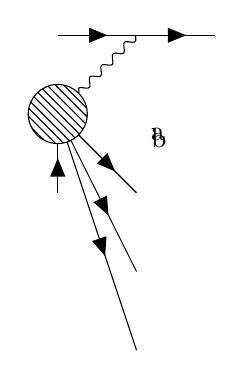
\begin{tikzpicture}
	\begin{feynman}
		\vertex (e1);
		\vertex [below right=of e1] (a){a};
		\vertex [right=of e1] (e2);
		\vertex [below right=of e1] (b){b};
		\vertex [below=of e1] (p);
		\vertex [below=of e2] (c);
		\vertex [below=of c] (d);
		\vertex [below=of d] (e);
		
		\diagram*[vertical'=a to b]{
			e1 -- [fermion] a -- [fermion] e2,
			a -- [photon] b [blob],
			p -- [fermion] b -- [fermion] {c,d,e},
		};	
	\end{feynman}
\end{tikzpicture}


\end{document}